	% NERMLAB Circuit and Mechanical Diagram
	
	\usetikzlibrary{calc,patterns,angles,quotes}
	
	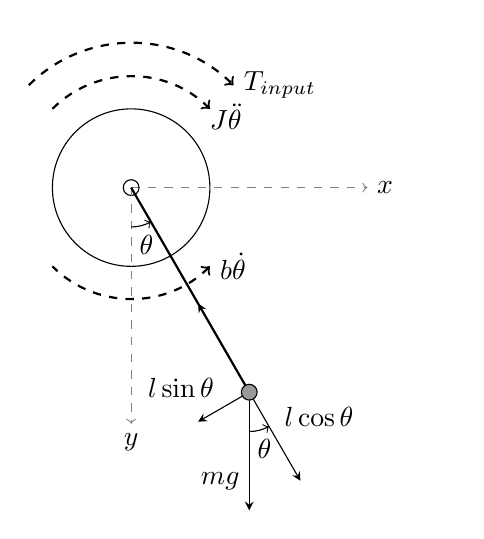
\begin{tikzpicture}[scale=1]	
 % save length of g-vector and theta to macros
 
 
 
\pgfmathsetmacro{\Gvec}{1.5}
\pgfmathsetmacro{\myAngle}{30}
% calculate lengths of vector components
\pgfmathsetmacro{\Gcos}{\Gvec*cos(\myAngle)}
\pgfmathsetmacro{\Gsin}{\Gvec*sin(\myAngle)}

\draw[->,dashed,gray] (0,0) -- ++ (3,0) node (mary) [black,right]{$x$};
\draw (0,0) circle (1cm);
\draw (0,0) circle (0.1cm);

\coordinate (centro) at (0,0);
\draw[->,dashed,gray] (centro) -- ++ (0,-3) node (mary) [black,below]{$y$};
\draw[thick] (centro) -- ++(270+\myAngle:3) coordinate (bob);
\pic [draw, ->, "$\theta$", angle eccentricity=1.5] {angle = mary--centro--bob};
\draw [black,-stealth] (bob) -- ($(bob)!\Gcos cm!(centro)$);
\draw [-stealth] (bob) -- ($(bob)!-\Gcos cm!(centro)$)
coordinate (gcos)
node[midway,above right] {$l\cos\theta$};
\draw [-stealth] (bob) -- ($(bob)!\Gsin cm!90:(centro)$)
coordinate (gsin)
node[midway,above left] {$l\sin\theta$};
\draw [-stealth] (bob) -- ++(0,-\Gvec)
coordinate (g)
node[near end,left] {$mg$};
\pic [draw, ->, "$\theta$", angle eccentricity=1.5] {angle = g--bob--gcos};
\filldraw [fill=black!40,draw=black] (bob) circle[radius=0.1];

\node[text width=3cm] at (2.5,0.9) {$J \ddot{\theta}$};
\draw [->, dashed, thick] (-1,1) to [out=45, in=135] (1,1); 
\draw [<-, dashed, thick] (1,-1) node[below,right]{$b \dot{\theta}$} to [out=-135, in=-45] (-1,-1) ; 
\draw [->, dashed, thick] (-1.3,1.3) to [out=45, in=135] (1.3,1.3) node[above,right]{$T_{input}$}; 
	\end{tikzpicture}